\documentclass[a4paper, 12pt]{report}
\usepackage[dvipsnames]{xcolor}
\usepackage{graphicx} % Required for inserting images
\usepackage{amsfonts}
\usepackage{amssymb}
\usepackage{tikz,lipsum,lmodern}
\usepackage[most]{tcolorbox}
\usepackage{pgfplots}
\usepackage{tabularx}
\usepackage{stmaryrd}
\usepackage{tikz} 
\usepackage{imakeidx}
\usepackage{blindtext}
\usepackage{hyperref}
\usepackage[rightcaption]{sidecap}
\usepackage{wrapfig}
\usepackage{cancel}

\hypersetup{
    colorlinks=true,
    linkcolor=black,
    filecolor=magenta,      
    urlcolor=blue,
    pdftitle={Relazione progetto e-commerce},
    pdfpagemode=FullScreen,
}

\setlength{\parindent}{0pt}
\setlength{\parskip}{5pt}


\makeindex[columns=3, title=Alphabetical Index, intoc]
\hypersetup{
    colorlinks=true,
    linkcolor=blue!50!green,
    filecolor=magenta,      
    urlcolor=cyan,
    pdftitle={Overleaf Example},
    pdfpagemode=FullScreen,
    }

\newcommand\scalemath[2]{\scalebox{#1}{\mbox{\ensuremath{\displaystyle #2}}}}
\definecolor{bananamania}{rgb}{0.98, 0.91, 0.71}
\definecolor{amaranth}{rgb}{0.9, 0.17, 0.31}
\definecolor{amethyst}{rgb}{0.6, 0.4, 0.8}
\definecolor{darktangerine}{rgb}{1.0, 0.66, 0.07}
\definecolor{cerise}{rgb}{0.87, 0.19, 0.39}
\definecolor{babyblue}{rgb}{0.54, 0.81, 0.94}


\title{Relazione su \\
Controllo formazione droni}
\author{A. Bettoni (1998044),\\ A. Coppola (2003964),\\S. Di Cesare (1938649)}
\date{\today}

\begin{document}
\maketitle
\newpage
\tableofcontents
\newpage
\chapter{Descrizione Generale}
Si vuole progettare un sistema di controllo di n droni che sorvegli una data area chiusa.

Il sistema gestisce una torre di controllo e ricarica, dalla quale i droni devono partire e devono tornare per ricaricarsi. 
I droni una volta connessi alla torre, seguono le sue indicazioni e si dirigono verso ogni punto gli venga assegnato dalla torre.
I droni seguono un sistema di volo "a tappe", in cui la torre invia loro una posizione indicata con delle coordinate cartesiane
relative alla dimensione dell'area da sorvegliare. Una volta che il drone arriva alla posizione ricevuta lo comunica alla torre che risponde con la posizione successiva, delineando così un percorso.
Quando il drone è scarico lo comunica alla torre e si direziona alla torre di controllo, per essere ricaricato.

Sta alla torre quindi il compito di calcolare, mentre i droni sono in volo, il percorso migliore per far sì che ogni punto dell'area venga sorvegliato 
il più frequentemente possibile, tenendo conto dei punti visitati, dei droni in volo, e dei punti che visitano prima di scaricarsi.
\newpage
\section{Idea dell'algoritmo}
Contando di avere un database con almeno \{\textit{Id, Posizione, Stato, Blocco}\} di tutti i droni che si sono connessi alla torre e le dimensioni dell'area da sorvegliare, la torre inizia a seguire il seguente algoritmo.

Definiamo $6$ stati in cui ogni drone può trovarsi:
\begin{enumerate}
    \item \textbf{Ready:} il drone è carico e si trova nella torre di controllo (è pronto a partire)
    \item \textbf{Starting:} il drone si sta posizionando verso il punto di partenza assegnatogli dalla torre di controllo
    \item \textbf{Flying:} il drone sta scansionando l'area che gli è stata assegnata seguendo i punti inviati dalla torre
    \item \textbf{Returning:} la carica del drone è sufficiente solo per il suo rientro 
    \item \textbf{Charging:} il drone si trova alla base, e sta ricaricando la sua batteria
    \item \textbf{Death:} la batteria del drone si è scaricata prima che questo potesse rientrare oppure la torre di controllo non riesce più a contattarlo.
\end{enumerate}
Il problema può essere gestito seguendo i seguenti passaggi:
\begin{enumerate}
    
    \item La torre di controllo conta i droni che si sono connessi e divide l'area da sorvegliare in $N$ blocchi tutti della stessa misura secondo una specifica funzione che fa in modo di avere $N \ge $numero dei droni.

    \item La torre assegna ad ogni drone \textit{Ready} un blocco.

    \item Ogni drone si dirige al punto di partenza stabilito assegnatogli dalla torre. Non appena lo raggiunge lo comunica alla torre.

    \item Quando la torre riceve il messaggio da un drone che si trova al punto di partenza del blocco, cambia il suo stato in \textit{Flying}.

    \item Quando un drone in stato \textit{Flying} si trova nel punto stabilito, la torre gli invia il punto successivo in base ad un semplice algoritmo di scanning del blocco.

    \item Quando la torre riconosce che un drone ha scansionato l'intero blocco assegnatogli, lo dissocia da tale blocco e glie ne assegna uno nuovo.\\ Quindi imposta il suo stato in \textit{Starting} e gli invia lo start del blocco. 

    \item Quando il drone raggiunge il punto di partenza il loop ricomincia dal punto $5$

    \item Quando il drone calcola che la batteria che gli rimane è appena sufficiente a rientrare alla torre invia un messaggio che segnala il suo rientro e si dirige nella posizione della torre di controllo.
    \\Quando la torre riceve il suo messaggio, mette il drone in stato di \textit{Returning} e modifica imposta lo start del blocco all'ultimo punto visitato dal drone.

    \item Quando il drone arriva alla torre di controllo viene messo in stato di \textit{Charging} e inizia a ricaricarsi.
    La torre gli assegnerà lo stato \textit{Ready} non appena la batteria sarà carica.

    \item Se la torre non riceve messaggi da un drone in volo per troppo tempo questo passa in stato \textit{Death}
\end{enumerate}
Questo è il ciclo principale che viene seguito finché il programma non viene interrotto da un operatore esterno o quando tutti i droni muoiono.

\section{Requisiti di sistema}
Per funzionare, il sisitema ha bisogno dei seguenti requisiti:
\begin{itemize}
    \item dimensione dell'area\\
    dato che l'area verrà divisa in blocchi, per ogni blocco è di interesse:
    \begin{itemize}
        \item limite alto superiore
        \item limite basso inferiore
        \item punto di partenza (o ultimo punto visitato)
    \end{itemize}
    \item numero di droni\\
    per ogni drone è di interesse:
    \begin{itemize}
        \item id: identificativo univoco seriale
        \item Stato : tra i stati precedentemente elencati
        \item posizione 
        \item carica residua (in minuti)
        \item carica massima (in minuti)
        \item tempo di ricarica 
        \item last\_update : tempo trascorso dall'ultimo update
    \end{itemize}
\end{itemize}
\newpage
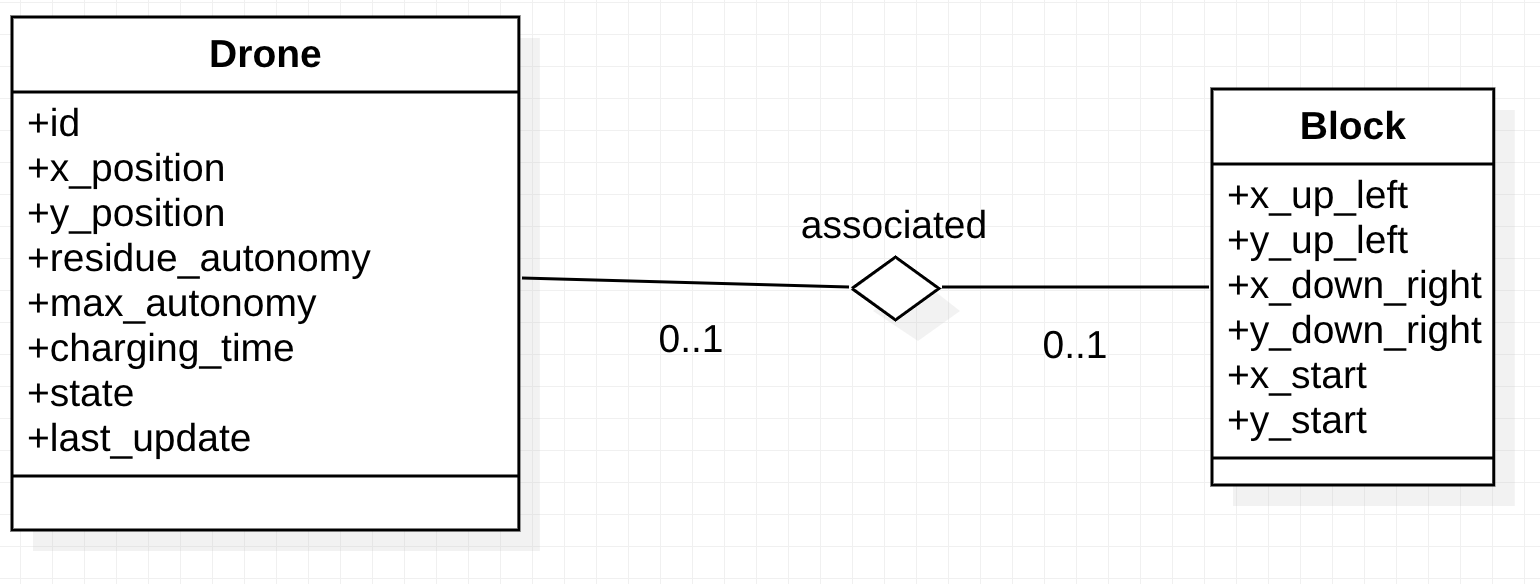
\includegraphics[height=6.25cm]{image/ER.png}\\
\


\end{document}